Le diagramme de cas d'utilisation offre une vue d'ensemble du système en représentant les interactions entre les acteurs et les cas d'utilisation correspondant aux principales fonctionnalités attendues. Il permet de définir les exigences fonctionnelles, de clarifier les objectifs du projet, de délimiter le périmètre du système et d’identifier les besoins des utilisateurs \cite{case}.

Dans ce diagramme, présenté à la figure \ref{fig:UseCaseDiagram1}, sont regroupés tous les cas d’utilisation de base afin d’offrir une perspective globale du fonctionnement de notre système.
\begin{figure}[H]
\centering
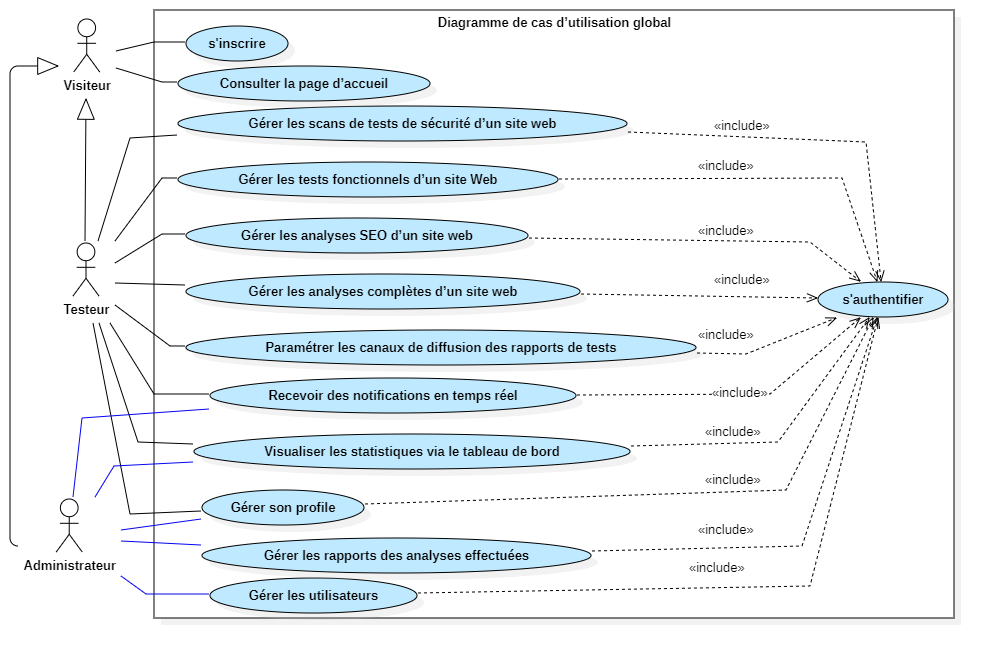
\includegraphics[width=\textwidth]{chapitres/ch2/img/global-last- use-case.png}
\caption{Diagramme de cas d'utilisation global}
\label{fig:UseCaseDiagram1}
\end{figure}
\vspace{-0.3cm}